\section{Imaging and Image Processing}

Considering prediction of brain activity requires that we look not only at the
current state of brain simulation, but also towards the future. A biological
brain processing the life of an organism, and a simulation of the same requires
that a link is made between the two: the state of the brain must be copied over as a
snapshot. This imaging process would likely take the form of an in vitro scan of
a preserved nervous system or some form of in vivo scan. These images would be
processed and turned into a model that could be simulated. Current techniques for imaging the brain give us some insight into to how this
uploading process might function and perform.

\subsection{Current Methods of Scanning the brain}

Given a 2D substrate such as a layer of brain tissue, there are several methods
of producing a high resolution image. These methods must balance the resolution
and noise levels required of model creation, with the speed with which the image
is taken \autocite{bostrom_whole_2008,mikula_progress_2016}.

\begin{figure}[h]
    \centering
    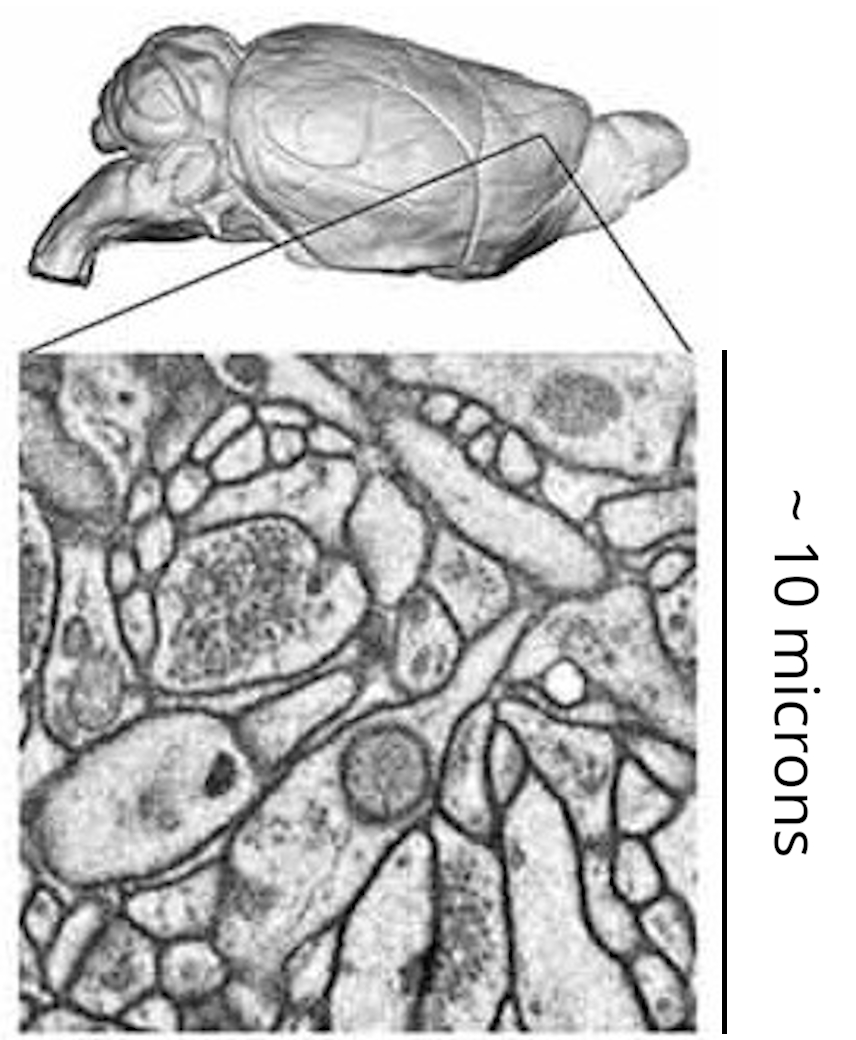
\includegraphics[scale=2]{figures/images/enlarge.jpg}
    \DoubleCaption{TODO Illustration of the scale of neurons in the brain.}
    {Adapted from \cite[fig. 1]{mikula_progress_2016}}
    \label{scaleexample}
\end{figure}
\vspace{1ex}

Given the level of emulation that is intended from a model, the images that
synthesise the model must resolve a minimum level of detail. In figure
\ref{scaleexample}, the general position of neuron somas 
% what be somas
and the rough links between them can be identified, but more subtle morphologies
of these links are missing. Perhaps another imaging method could resolve further
detail. The specifications and drawbacks of several imaging methods are
described below.

\subsubsection*{MRI}

Magnetic Resonance Imaging (MRI) scanning is a common medical procedure, and can
be used to provide information about the regions of the brain and general
connective patterns between these regions. However, at current generally
available resolutions, MRI is not suitable for reconstructing any kind of neural
model that contains information pertaining to discrete connections between
neurons. Future technologies that enable brain emulation of the
biologically alive would need to offer a similar feature set as MRI scanning
whilst producing images many thousands of times more detailed. Such MRI
microscopy does exist currently, but is significantly more limited in scale,
scanning small chunks of cortical tissue at a very high resolution
\autocite{johnson_three-dimensional_1987,bostrom_whole_2008}.

\subsubsection*{Electron Microscope Scanning}

Electron Microscopy (EM) is a commonly used technology in any discipline where
one may wish to resolve detail at the scale of nano-metres. Since the wavelength
of accelerated electrons is much shorter than the wavelength of visible light,
the resolution of EM is not limited by diffraction in the same way as optical
imaging. As a result, it is the imaging method of choice for neural and cortical
tissue \autocite{marc_retinal_2013, kaynig_large-scale_2015}. EM is not without
drawbacks however, as brain tissue must be chemically preserved before
processing, making it a complicated and expensive procedure. 

One variation of EM is Correlative Light-Electron Microscopy (CLEM) which takes
a hybrid approach to imaging the brain with both optical and electron imaging.
CLEM therefore has the advantage of accurate recognition of cell types from the
optical sensor, while the electron component provides the resolution required to
determine structure. Correlating images from both sensors requires alignment
through expensive computational techniques \autocite{voortman_integration_2014}.

%  - precise
%  - long time
%  - freeze or measurement drift

\subsection{Connectomics and network modelling}
Connectomics is the production and study of connectomes, using electron
microscopy images from layers of tissue to map complex neural networks
\autocite{marc_retinal_2013}. This process can have many stages depending on the
desired complexity of the connectome. 

\begin{figure}[h!]
    \centering
    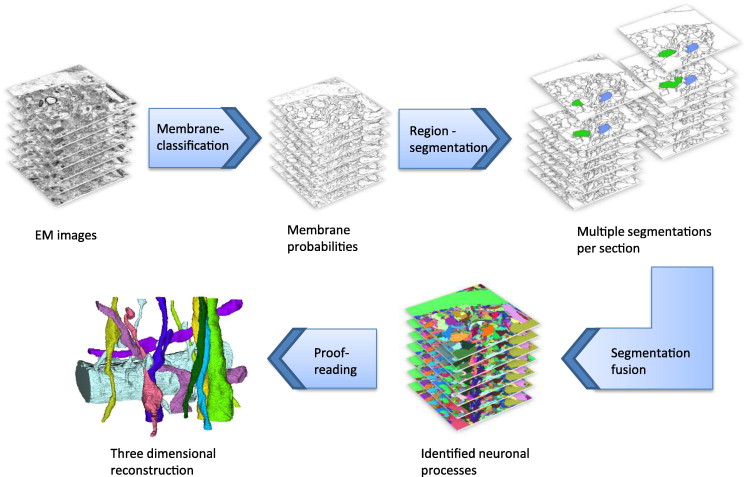
\includegraphics[scale=0.75]{figures/images/reconstruction.jpg}
    \DoubleCaption{TODO Illustration of a typical workflow for connectome
        reconstruction}
    {Reproduced from \cite{kaynig_large-scale_2015}}
    \label{reconstruction}
\end{figure}
% \vspace{1ex}

A typical workflow for constructing
connectomes is shown in figure \ref{reconstruction}, where large datasets
produced from EM are processed and fused to create a 3D connectome that
re-creates the original observed connectivity, complete with cellular metadata
if enough detail has been resolved. This process is limited by the time and
manual tuning required to process these EM datasets however, as automated
algorithms for processing can produce errors, and the reliability of the
connectome is limited by the quality of the EM data used to create it. 
\autocite{pallotto_extracellular_2015} In
particular, the recognition and reconstruction of network morphology is
especially hard to automate reliably \autocite{helmstaedter_connectomic_2013}.

\subsection[Error induced through noise]{Examination of Error induced through the imaging process}

Prediction of future brain activity through simulation requires an accurate and
detailed connectome of a brain, with synapses and neurons correctly located in
space and the metadata of each neuron in the system replicated with minimal
error \autocite{bostrom_whole_2008}. The accuracy of such a model depends on the
resolution of the imaging method used to create it, and the error resulting from
such a imaging method is the measurement error. Depending on imaging procedure, brain matter may shift in composition during the course of the scan, which is the cause of measurement drift, itself a form of measurement error.

\setlength{\tabcolsep}{4ex}
\renewcommand{\arraystretch}{1.1}
\begin{table}[ht]
    \centering
    \begin{tabular}{@{}llll@{}}
        Method              & Resolution                 & Time    & Error(approx.) \\
        \hline
        MRI                 & 6$\mu m$                   & 30mins  & 95\%           \\
        MRI microscopy      & 3$\mu m$                   & -       & 85\%           \\
        XRay microscopy     & 30nm                       & -       & 30\%           \\
        Electron microscopy & \textasciitilde 30nm-0.1nm & >3mnths & <1\%           \\
        Theoretical Ideal   & <5nm                       & <500s   & <1\%           \\
        \hline
    \end{tabular}
    \DoubleCaption{Comparison of imaging methods.}{Error approximated from size of dendritic spines.}
    \label{imagemethodcomparison1}
\end{table}
\setlength{\tabcolsep}{1ex}

In the above table \ref{imagemethodcomparison1}, I have summarised each of the
major methods that could be considered for imaging the whole human brain. The
theoretical ideal represents the requirements for an imaging process that would
enable the mass creation of connectomes, as a technical requirement of uploading
general human consciousness to vast simulations. These error values will form
the basis of the model and simulation that is described and evaluated later in
this document.
